\section{Auswertung}
Die in der Auswertung bestimmten Ausgleichsrechnungen werden mit
dem Python Paket \emph{scipy.optimize} berechnet.

\subsection{Bestimmung von RC mithilfe der Entladekurve}

Das für die Berechnung benötigte Ozsilloskopenbild ist in Abbbildung \ref{fig:entladekurve} zusehen.

\begin{figure}
  \centering
  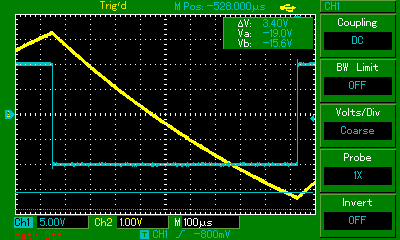
\includegraphics[width=0.5\textwidth]{pics/bilda_508hz.png}
  \caption{Vom Ozsillopskop gespeicherte Entladekurve.}
  \label{fig:entladekurve}
\end{figure}
Von dem Graphen wurden $9$ Punkte vermessen.
Diese sind in Tabelle \ref{fig:plot_teila} eingetragen.
\FloatBarrier
\begin{table} 
\centering 
\caption{Aus der Grafik \ref{fig:entladekurve} bestimmte Messwerte} 
\label{tab:teil_a_spannungen} 
\begin{tabular}{S S } 
\toprule  
{$t$ in $\si{\milli\second}$} & {$U\ua{ein}$ in $\si{\volt}$}  \\ 
\midrule  
 0.0  & 6.0\\ 
0.1  & 5.2\\ 
0.2  & 4.4\\ 
0.3  & 3.7\\ 
0.4  & 3.0\\ 
0.5  & 2.3\\ 
0.6  & 1.8\\ 
0.7  & 1.3\\ 
0.8  & 0.8\\ 
\bottomrule 
\end{tabular} 
\end{table}

\FloatBarrier
An die Messwerte wird ein Fit der Form

\begin{equation*}
  U(t)=a\map{e}^{bt}+c.
\end{equation*}

gelegt.
Als Parameter ergeben sich:
\begin{equation}
  \label{eq:parameter_teila}
a=\SI{11.3\pm0.7}{\volt} \quad b=\num{-780.5\pm67.7} \quad c=\SI{-5.3\pm0.7}{\volt}.
\end{equation}
Aus der Formel  \eqref{eq:entlade_kurve} folgt weiter
\begin{equation}
  \frac{1}{b}=RC=\SI{1.12\pm0.1}{\milli\second}.
\end{equation}
Die Messwerte und der Fit sind in Abbildung \ref{fig:plot_teila}  graphisch
dargestellt.


\begin{figure}
  \centering
  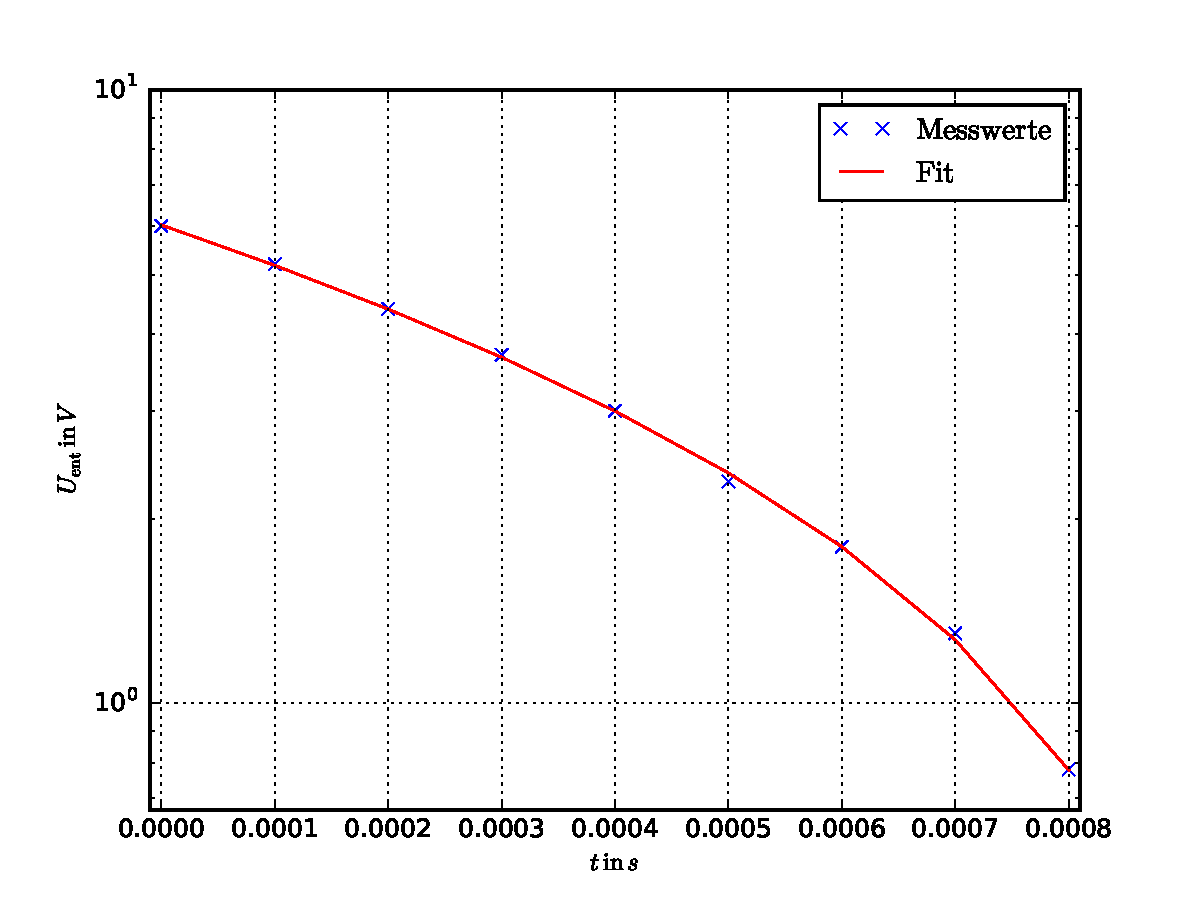
\includegraphics [width=0.8\textwidth]{pics/teil_a_entladung.pdf}
  \caption{Messwerte und Fit der Entladekurve}
  \label{fig:plot_teila}
\end{figure}
\subsection{Bestimmung von RC mithilfe der Kondensatorspannung}
Im Versuch wurden die in \ref{tab:teil_b_spannungen} dargestellten Werte gemesen.

\begin{table} 
\centering 
\caption{Gemessene Generator- und Kondensatorspannungen bei unterschiedlichen Frequenzen } 
\label{tab:teil_b_spannungen} 
\begin{tabular}{S S S S } 
\toprule  
{$f$ in $\si{\hertz}$} & {$U\ua{g}$ in $\si{\volt}$}& {$U\ua{C}$ in $\si{\volt}$} & {$\frac{U\ua{C}}{U\ua{g}}$}  \\ 
\midrule  
 11  & 10.29  & 10.29  & 1.00\\ 
25  & 10.29  & 9.90  & 0.96\\ 
50  & 10.29  & 9.21  & 0.89\\ 
75  & 10.29  & 8.41  & 0.82\\ 
100  & 10.29  & 7.37  & 0.72\\ 
200  & 10.39  & 4.95  & 0.48\\ 
401  & 10.29  & 2.81  & 0.27\\ 
600  & 10.29  & 1.94  & 0.19\\ 
800  & 10.29  & 1.38  & 0.13\\ 
1000  & 10.29  & 1.11  & 0.11\\ 
1200  & 10.29  & 0.93  & 0.09\\ 
1400  & 10.29  & 0.77  & 0.07\\ 
1600  & 10.29  & 0.71  & 0.07\\ 
1800  & 10.29  & 0.64  & 0.06\\ 
2000  & 10.29  & 0.57  & 0.06\\ 
2500  & 10.29  & 0.47  & 0.05\\ 
3000  & 10.29  & 0.40  & 0.04\\ 
3500  & 10.29  & 0.32  & 0.03\\ 
4000  & 10.29  & 0.28  & 0.03\\ 
\bottomrule 
\end{tabular} 
\end{table}


In diesem ist zugleich die Nomierung $\frac{U\ua{c}}{U\ua{g}}$
mitangegben.
Mit der Formel \eqref{eq: amplitude_theorie} kann an die Messwerte eine Regressionsgerade
errechnet werden. Hierbei wurde der Zusammenhang $\omega=2\pi f$ genutzt.
Aus der Regerssionsrechung folgt für den Wert von $RC$:
\begin{equation}
  \label{eq:rc_teilb}
  RC=\SI{1.49\pm0.02}{\milli\second}.
\end{equation}
In der Abbildung \ref{fig:teilb} sind Messwerte und Regressionsgerade abgebildet.

\begin{figure}
  \centering
  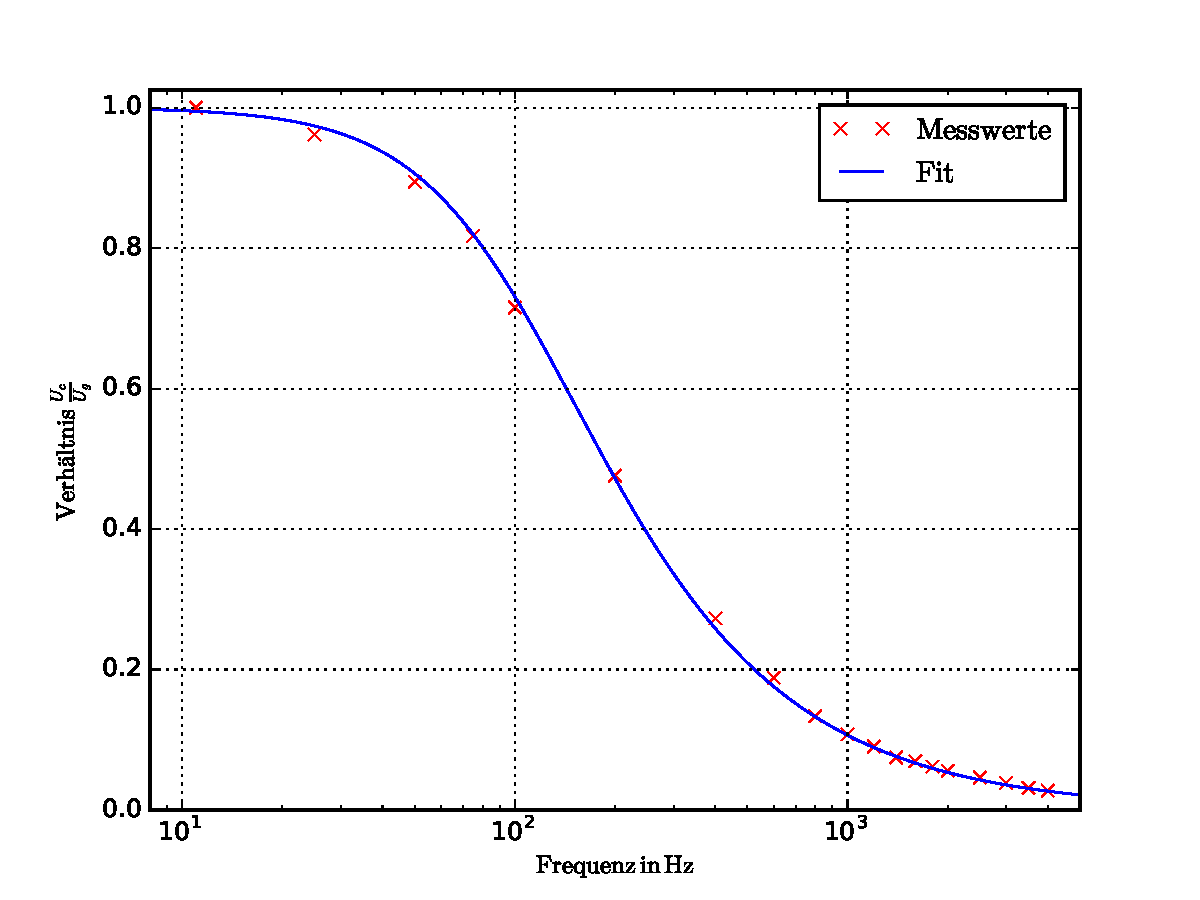
\includegraphics[width=0.8\textwidth]{pics/u_cdurchu_g.pdf}
  \caption{Normierte Amplitude in Abhängigkeit von der Frequenz.}
  \label{fig:teilb}
\end{figure}

\subsection{Bestimmung von RC mithilfe der Phasenverschiebung}
Die im Versuch gemessenen Abstände $a$ und $b$ in Tabelle \ref{tab:teil_c_abstaende}
dargestellt. Mithilfe von Formel \eqref{eq:phasenverschiebung} wurde die
Phasenverschiebung bestimmt.

\begin{table} 
\centering 
\caption{Gemessene Abstände $a$ und $b$ } 
\label{tab:teil_c_abstände} 
\begin{tabular}{S S S S } 
\toprule  
{$f$ in $\si{\hertz}$} & {$a$ in $\si{\milli\second}$}& {$b$ in $\si{\milli\second}$ }& {$\varphi$}  \\ 
\midrule  
 11  & 1.280  & 91.00  & 0.09\\ 
25  & 1.280  & 39.83  & 0.20\\ 
50  & 1.380  & 19.98  & 0.43\\ 
75  & 1.240  & 13.29  & 0.59\\ 
100  & 1.160  & 9.99  & 0.73\\ 
200  & 0.880  & 4.98  & 1.11\\ 
401  & 0.504  & 2.48  & 1.28\\ 
600  & 0.380  & 1.67  & 1.43\\ 
800  & 0.304  & 1.25  & 1.53\\ 
1000  & 0.244  & 1.00  & 1.53\\ 
1200  & 0.208  & 0.83  & 1.57\\ 
1400  & 0.190  & 0.71  & 1.67\\ 
1600  & 0.168  & 0.62  & 1.69\\ 
1800  & 0.150  & 0.56  & 1.70\\ 
2000  & 0.140  & 0.50  & 1.76\\ 
2500  & 0.114  & 0.40  & 1.80\\ 
3000  & 0.111  & 0.33  & 2.10\\ 
3500  & 0.097  & 0.28  & 2.14\\ 
4000  & 0.088  & 0.25  & 2.22\\ 
\bottomrule 
\end{tabular} 
\end{table}


Es fällt auf das die Phase $\varphi$ größer als $\frac{\pi}{2}$ wird.
Dies ist nach der Theorie nicht möglich.
Es lässt sich also schon jetzt ein systematischer Fehler nicht ausschließen.
Deshalb werden für die Berechnung von $RC$ die Messwerte weggelassen, an den
$\varphi$ größer als $\frac{\pi}{2}$ ist.
Mit der Gleichung \eqref{eq: phase_theorie} kann eine Regressionskurve für die
Phase bestimmt werden.
In Abbildung \ref{fig:plot_teil_c} sind Messwerte und Regressionskurve aufgetragen.
Dabei wird einmal die Regressionskurve mit und einmal ohne Korrekur abgebildet.

\FloatBarrier
\begin{figure}
  \centering
  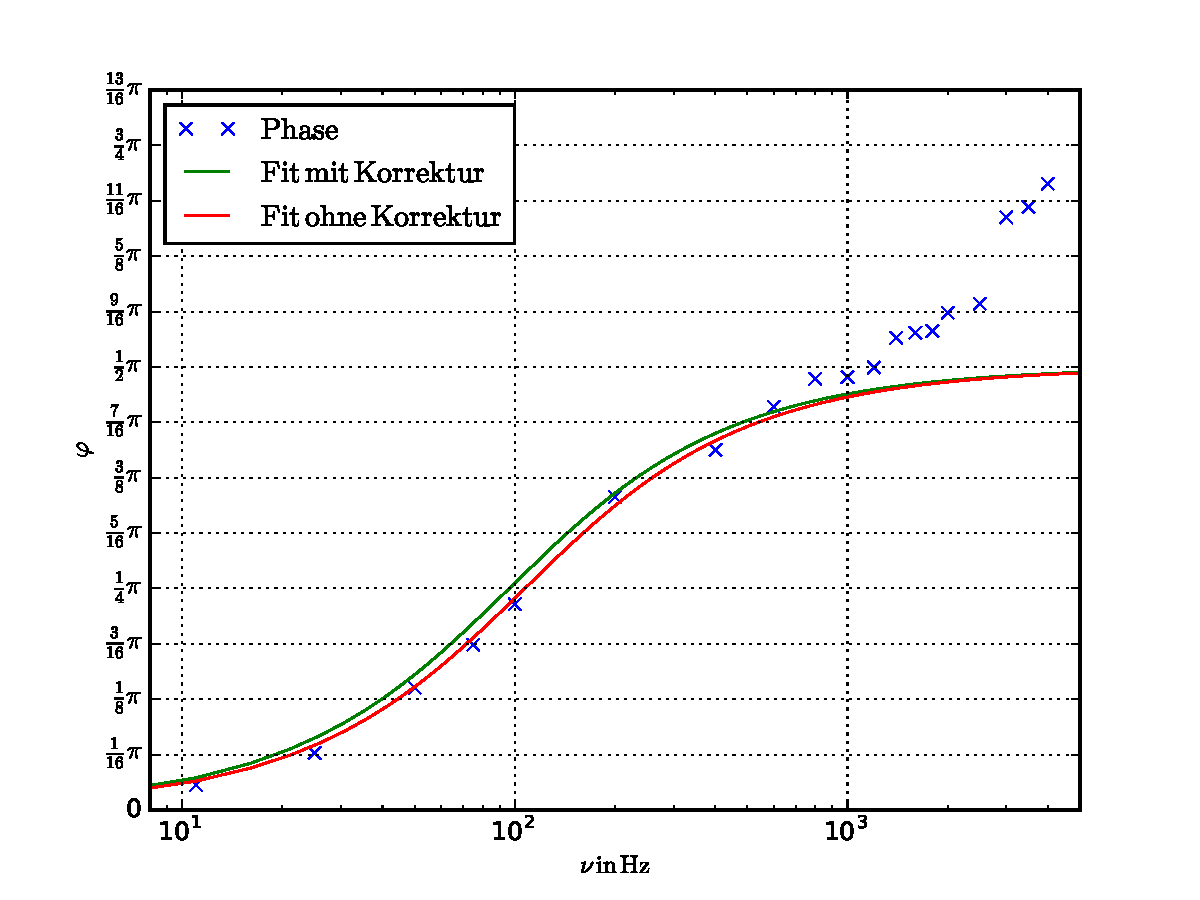
\includegraphics[width=0.8\textwidth]{pics/frequenz_phase.pdf}
  \caption{Die von der RC-Kombination erzeugte Phasenverschiebung.}
  \label{fig:plot_teil_c}
\end{figure}
\FloatBarrier

Aus der Regressionsrechung ergibt sich als Wert für $RC$

\begin{align}
  \label{eq:teil_c_rc}
  \begin{aligned}
    RC&=\SI{1.7\pm0.5}{\milli\second} \quad \text{ohne Korrektur} \\
    RC& =\SI{1.49\pm0.07}{\milli\second} \quad \text{mit Korrektur}.
\end{aligned}
\end{align}

\subsection{Phasenabhängigkeit der Kondensatorsspanung}

Für die Berechnung der Amplitude wird angenommen das $RC=\SI{1.49\pm0.07}{\milli\second}$
groß ist. Es kann dann mithilfe von \eqref{eq:phase} die Amplitude aus den Messwerten bestimmt werden.
Diese sind in Tabelle \ref{tab:teil_d_amplitude} aufgelistet und in Abbildung \ref{fig:plot_teil_d} dargestellt.
\FloatBarrier
\begin{table} 
\centering 
\caption{Berechnete normierte Amplitude bei $RC =\SI{1.49}{\milli\second}$} 
\label{tab:teil_d_amplitude} 
\begin{tabular}{S S S } 
\toprule  
{$f$ in $\si{\hertz}$} & {$\varphi$}& {$\frac{U\ua{C}}{U\ua{g}}$}  \\ 
\midrule  
 11  & 0.09  & 0.86\\ 
25  & 0.20  & 0.86\\ 
50  & 0.43  & 0.90\\ 
75  & 0.59  & 0.79\\ 
100  & 0.73  & 0.71\\ 
200  & 1.11  & 0.48\\ 
401  & 1.28  & 0.25\\ 
600  & 1.43  & 0.18\\ 
800  & 1.53  & 0.13\\ 
1000  & 1.53  & 0.11\\ 
1200  & 1.57  & 0.09\\ 
1400  & 1.67  & 0.08\\ 
1600  & 1.69  & 0.07\\ 
1800  & 1.70  & 0.06\\ 
2000  & 1.76  & 0.05\\ 
2500  & 1.80  & 0.04\\ 
3000  & 2.10  & 0.03\\ 
3500  & 2.14  & 0.03\\ 
4000  & 2.22  & 0.02\\ 
\bottomrule 
\end{tabular} 
\end{table}

\FloatBarrier
\FloatBarrier
\begin{figure}
  \centering
  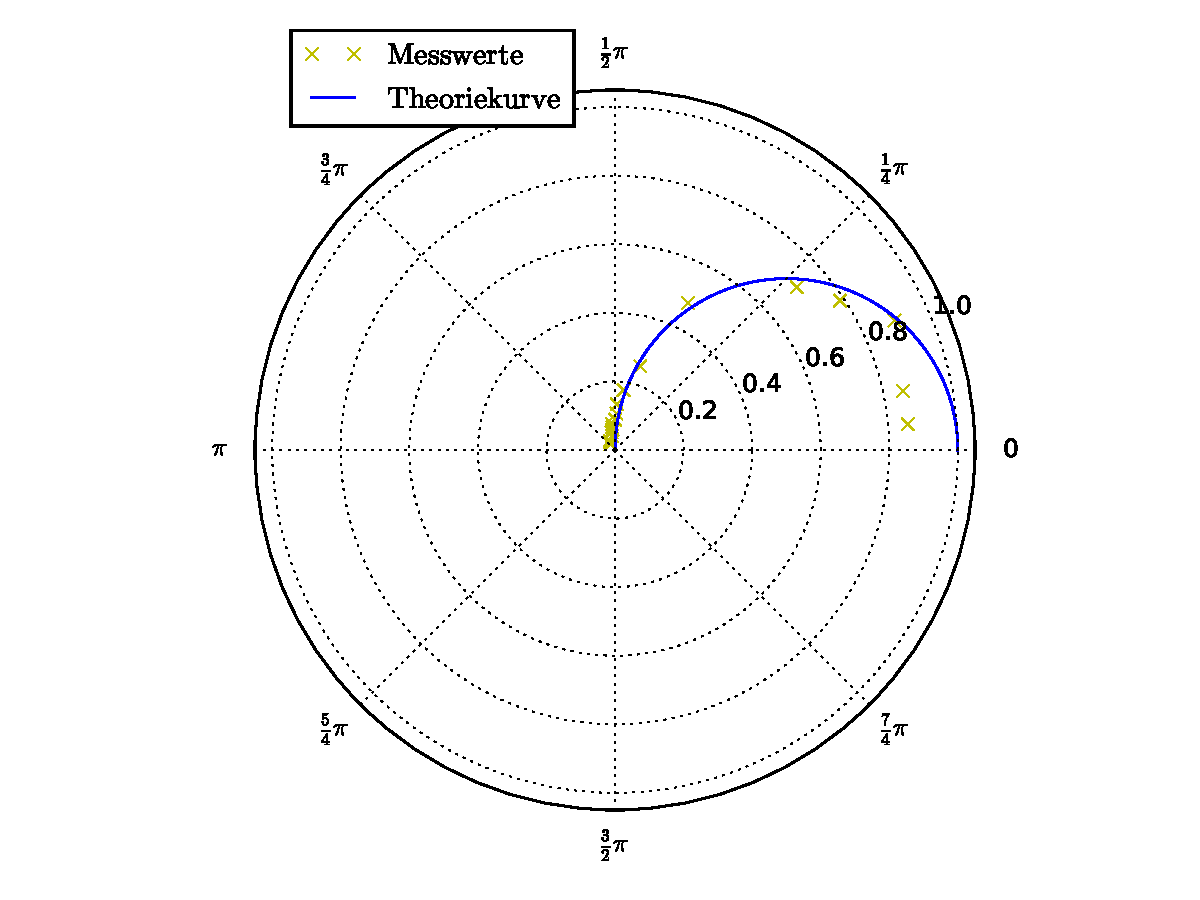
\includegraphics[width=0.8\textwidth]{pics/polarplot.pdf}
  \caption{Die normierte Amplitude in Abhängigkeit von der Phase.}
  \label{fig:plot_teil_d}
\end{figure}
\FloatBarrier

Die Theoriekurve kann mit Gleichung \eqref{} bestimmt werden.

\subsection{Der RC-Kreis als Integrator}

Wie in der Theorie erwähnt kann ein $RC$-Kreis genutzt werden, um eine
Spannung zu integrieren.
Dieser Effekt wird an jeweils Rechteck-, Sinus- und Dreicksspannungen
überprüft.
In den Abbildungen \ref{fig:rechteck}, \ref{fig:dreieck} und \ref{fig:sinus} sind die vom
Generator erzeugten Spannung (blau) und die integrierte Spannung
des RC-Gliedes (gelb) zusehen.
\FloatBarrier
\begin{figure}
  \centering
  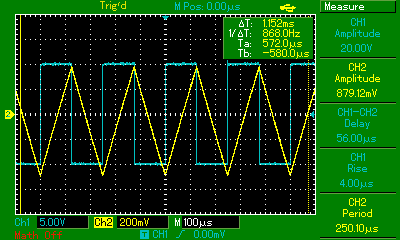
\includegraphics[width=0.5\textwidth]{pics/teild_rechteckspannung.png}
  \caption{Rechtecksapnnung.}
  \label{fig:rechteck}
\end{figure}
\begin{figure}
  \centering
  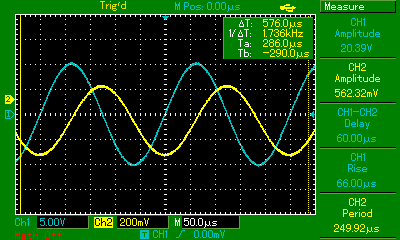
\includegraphics[width=0.5\textwidth]{pics/bildd_sinus.png}
  \caption{Sinusspannung}
  \label{fig:sinus}
\end{figure}
\begin{figure}
  \centering
  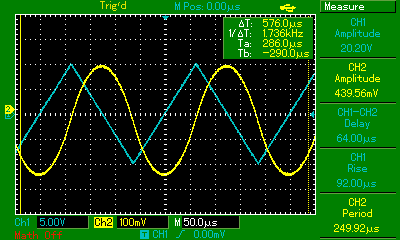
\includegraphics[width=0.5\textwidth]{pics/teild_dreieck.png}
  \caption{Dreiecksspannung}.
  \label{fig:dreieck}
\end{figure}
\FloatBarrier

Bei der in Abbildung \ref{fig:rechteck} zusehenden Rechteckspannung,
handeld es sich um eine konstante Spannung. Folglich müsste das Integrieren
eine Gerade hervor bringen:
\begin{equation*}
   \int\!\!\!c \dv{x}= cx+b \quad c,b\in\mathbb{R}.
\end{equation*}
Und in der Tat in der Abbildung ist als integriertse Spannung eine Gerade zu erkennen.

In Abbildung \ref{fig:dreieck} handelt es sich um eine Dreieckspannung (lineare Spannung),
diese sollte integriert eine quadratische Funktion ergeben.
\begin{equation*}
   \int\!\!\! mx+b \dv{x}= \frac{1}{2}mx^2+bx+c \quad m,b,c\in\mathbb{R}.
\end{equation*}
Die gelbe Spannung ist als eine solche identifizierbar.
Zu letzt ist in Abbildung \ref{fig:sinus} die Generatorspannung sinusförmig.
Die Stammfunktion vom Sinus ist:
\begin{equation*}
  \int\!\!\! \sin(x)\dv{x}=-\cos(x)+c \quad c\in \mathbb{R}.
\end{equation*}
Der gelbe Spannungsverlauf besitzt diese Form.
